\section{Implementation Details}\label{sec:implementation}
% \begin{itemize}
%   \item Extension of the library RxLua
%   \item Why reactive?
%     \url{http://www.reactivemanifesto.org/}
%   \item ØMQ \textsc{Lua} bindings
%   \item ØMQ queues with push/pull protocol - Fire-and-forget messaging: a messsaging pattern in which we do not expect a direct response to the message, as opposed to request-response protocols
% \end{itemize}

%On September 2014 has been published the Reactive Manifesto\cite{reactivemanifesto}.
%This one attempts to define the principles to build systems more flexible, loosely-coupled and scalable.
%A \textit{reactive system} has to follow the four Reactive Principles:
%
%\begin{itemize}
%  \item Responsive: it is quick to react to all users in order to ensure a consistently positive user experience;
%  \item Elastic: it is easily upgraded on demand in order to ensure responsiveness under various load conditions;
%  \item Resilient: it applies proper design and architecture principles in order to ensure responsiveness;
%  \item Message-driven: it is based on a message-passing architecture to establish a boundary between components that ensures loose coupling, isolation and location transparency, e.g. event-driven, actor-based, or both of them.
%\end{itemize}
%
%The responsiveness of a system needs both elasticity and resiliency.
%Finally, a message-driven architecture is the foundation of elastic, resilient and responsive systems, as shown on figure \ref{fig:reactive-traits}.
%
%\begin{figure}[t!]
%  \centering
%  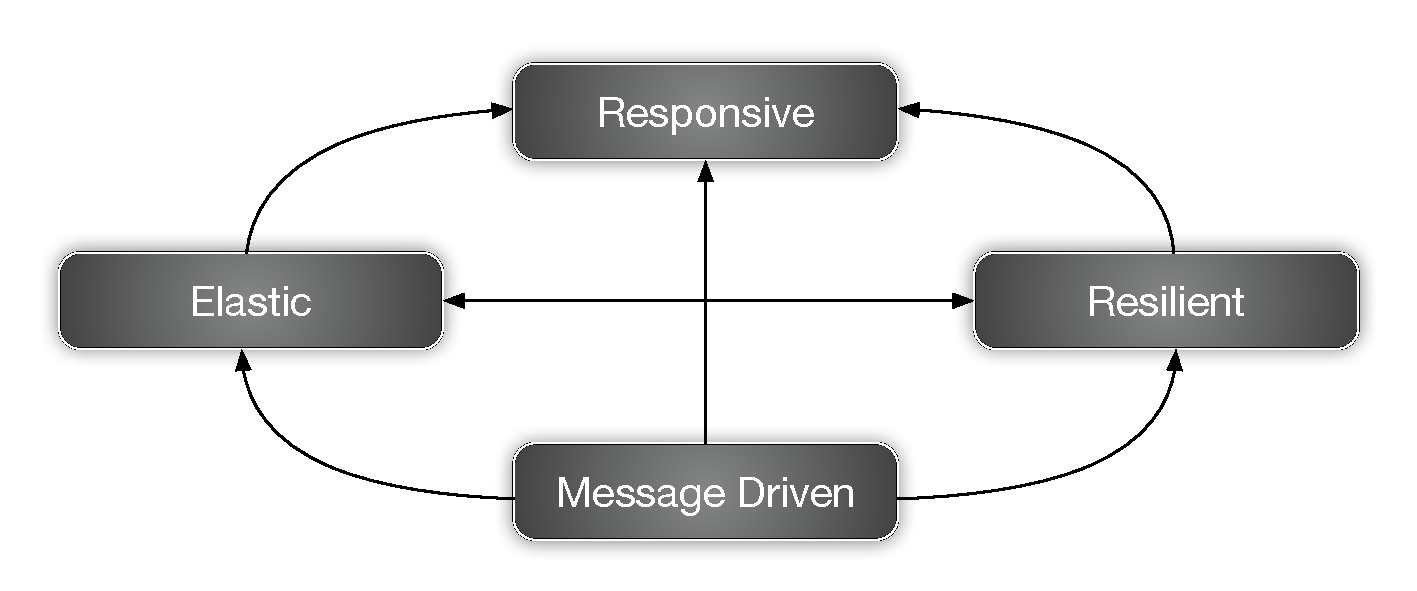
\includegraphics[width=.99\linewidth]{images/reactive-traits}
%  \caption{Reactive traits.}
%  \label{fig:reactive-traits}
%\end{figure}
%
%
%The term \textit{reactive} is not new in the field of computer sciences: Gérard Berry used it in 1989 while talking about \textit{real-time programming}\cite{berry:realtime_programming}.
%But recently the industry recognized the \textit{reactive paradigm} as the de facto way forward in system design\cite{malawski:why_reactive}.
%In the field of data streams, \textit{reactive programming} is programming with asynchronous streams, anything else.
%A stream is a sequence of ongoing events ordered in time, and these emitted events are captured only asynchronously by defining three functions:
%
%\begin{itemize}
%  \item an \textbf{onNext} function that will execute when a value is emitted;
%  \item an \textbf{onError} function executed when an error is emitted;
%  \item and finally an \textbf{onComplete} function executed when the stream is over.
%\end{itemize}
%
%
%
%A plenty of software libraries for different languages ensues from this paradigm\cite{reactive_streams}\cite{github:reactive_streams}.
%As exposed in section \ref{sec:architecture}, we chose the \textsc{Lua} technology as the basic of \SYS's implementation.
%Lua is a scripting language that is simple, efficient, extensible, functionnal and open-source\cite{ierusalimschy_programming_2006}.
%It will be easy to handle for the end user of \SYS.
%By the way, it is embedded in many application programs, such as Adobe Lighroom, Nmap, World of Warcraft or Nginx.

\SYS{} is implemented in \textsc{Lua} (v5.3).
Our implementation is compact, as it consists of only $120$ lines of code (without counting the dependencies).
The framework partially extends \rxl~\cite{github:rxlua}, a library for reactive programming in \textsc{Lua}.
\rxl provides to the developer the required API to design a data stream processing pipeline following a dataflow programming pattern~\cite{uustalu_essence_2005}.
Listing~\ref{pipeline-example} provides an example of a \rxl program (and consequently, a \SYS{} program) to compute the average age of a population by chaining \texttt{:map}, \texttt{:filter} and \texttt{:reduce} functions.
The \texttt{:subscribe} function performs the subscription of 3 functions to the data stream.
Following the \emph{observer} design pattern~\cite{szallies_using_1997}, these functions are observers, while the data stream is an observable.
%These functions are observers, and the stream is an observable: this is precisely an implementation of the \textit{Observer Design Pattern}~\cite{szallies_using_1997}.
%A simple program example, computing from a source of \textit{people} the average age of the adult ones, throw a map/filter/reduce pipeline, is presented in listing \ref{pipeline-example}.

%\begin{minipage}{\linewidth}
\begin{lstlisting}[language=LUA,caption={Example of process pipeline with RxLua.},label=pipeline-example]
Rx.Observable.fromTable(people)
 :map(
   function(person)
     return person.age
   end
 )
 :filter(
   function(age)
     return age > 18
   end
 )
 :reduce(
   function(accumulator, age)
     accumulator[count] = (accumulator.count
       or 0) + 1
     accumulator[sum] = (accumulator.sum
       or 0) + age
     return accumulator
   end
 )
 :subscribe(
   function(datas)
     print("Adult people average:",
       datas.sum / datas.count)
   end,
   function(err)
     print(err)
   end,
   function()
     print("Process complete!")
   end
 )
\end{lstlisting}
%\end{minipage}

\SYS{} dynamically ships the business logic for each component into a dedicated Docker container and executes it.
%Our extension takes the business logic in each element of the pipeline to send and execute it in a Docker container.
The communication between the Docker containers (the router and the worker components) happens through \zmq (v4.1.2) and the corresponding \textsc{Lua} bindings~\cite{github:lzmq}.
%Then, the data is streamed accross the network communication built on top of the ØMQ protocol and implemented using the ØMQ \textsc{Lua} bindings\cite{github:lzmq}.
Basically, \SYS{} abstracts the underlying network and computing infrastructure from the developer, by relying on \zmq and Docker.


\vspace{10pt}\noindent\textbf{\textsc{LuaVM} inside SGX.}
Under the SGX threat model where the system software is completely untrusted, system calls are not allowed inside secure enclaves.
By consequence, porting legacy applications or runtime, such as the \textsc{Lua} interpreter, is challenging.
%That makes porting legacy applications, like the \textsc{Lua} interpreter, more effortful.
To achieve it, we traced, all system calls made by the interpreter to the standard C library and replaced them by mock implementations that either mimic the real behavior or just do nothing.
Our changes to the vanilla \textsc{Lua} source code consist in the addition of about $600$ lines of code, or 2.5\% of its total size.
By doing so, \textsc{Lua} programs operating on files, network sockets or any other input/output device do not execute as they normally do outside the enclaves. %That means that pieces of script code that is meant to run inside enclaves will not perform as they were supposed to if they work on files, network sockets or use any other input/output instruction.
This inherent SGX limitation also reinforces the system security guarantees offered to the application developers.
%Despite being a limitation, this approach also reinforces security. 
The \SYS{} framework safely ships the data and code to enclaves.
Hence, the \textsc{Lua} scripts executed within the SGX enclave do not use (read/write) files or sockets.
Wrapper functions are nevertheless installed in the SGX-enabled \textsc{LuaVM} to prevent any of such attempts.
%Even if it does, that will be caught by the inocuous mock functions and make the attempt harmless.

An additional constraint imposed by the secure SGX enclaves is the impossibility of dynamically linking code. 
The reason is that the assurance that a given code is running inside a SGX-enabled processor is made through the measurement of its content when the enclave is created.
More specifically, this measurement is the result of \texttt{EREPORT} instruction, an SGX-specific report.
Despite the lack of documentation, we believe it computes a cryptographically secure hash of code, data and a few data structures, that overall builds a snapshot of the state of the enclave (including threads, memory heap size, etc.) and the processor (security version numbers, keys, etc.).
%\rp{Based on that measurement, further attestation mechanisms which ultimately allows them to receive sensitive information, such as the keys with which sensitive data will be thereafter exchanged.}\vs{i don't understand this. to rephrase}\rp{Attestation allows enclaves to receive secrets (like keys). Attestation is based on the 'measurement' of EREPORT. Clearer? $:)$} 
Allowing more code to be linked dynamically at runtime would break the assurance given by the attestation mechanism on the integrity of the code being executed, allowing for example an attacker to load a malicious library inside the enclave.
%If additional code were allowed, that assurance would no longer hold, which would render the system exploitable by malicious attackers.
In the case of \textsc{Lua}, a direct consequence is the impossibility of loading \textsc{Lua} extensions using the traditional dynamic linking technique. 
Every extension has to be statically compiled and packed with the enclave code. 
To ease the development of \SYS applications, we statically compiled \emph{json}~\cite{rfc7159} and \emph{csv}~\cite{rfc4180} parsers within our enclaved \textsc{Lua} interpreter.
With these two library, the size of the VM and the complete runtime remains reasonably small, approximately $220\,KB$ ($19\,\%$ larger than the original).

\begin{figure}[t!]
  \centering
  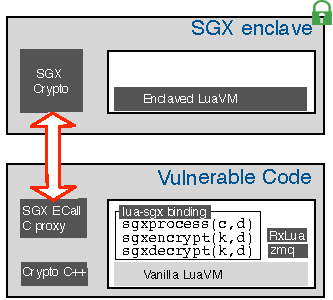
\includegraphics[width=.9\linewidth]{images/arch-sgxlua}
  \caption{Integration between \textsc{Lua} and Intel SGX.}
  \label{fig:arch-luasgx}
\end{figure}


While this restricted \textsc{Lua} has been adapted to run inside SGX enclaves, we still needed to provide a support for communications and the reactive streams framework itself.
To do so, we use an external vanilla \textsc{Lua} interpreter, with a couple adaptations that allowed the interaction with the SGX enclaves and the \textsc{LuaVM} therein.
Figure~\ref{fig:arch-luasgx} shows the conceived architecture.
We extend the \textsc{Lua} interface with 3 functions: \texttt{sgxprocess}, \texttt{sgxencrypt} and \texttt{sgxdecrypt}. 
The first forwards the encrypted code and data to be processed in the enclave, while the remaining two provide cryptographic functionalities.
In this work, we assume that attestation and key establishment was previously and correctly operated.
As result, safe key happens to be inside the enclave.
We plan to release our implementation as open-source.\footnote{Omitted due to DEBS17 double-blind policy.}
